\documentclass[11pt, letterpaper]{article}

\title{Assignment1: Questions 1 - 3}
\author{Stuart Mashaal}
\date{Sunday, October 1, 2017}

\usepackage[utf8]{inputenc}
\usepackage[margin=0.75in]{geometry}
\usepackage{graphicx}
\usepackage{indentfirst}
\usepackage{amsmath}
\usepackage{minted}

\begin{document}
\maketitle

\section*{Question 1}

Uniprogramming is a computing paradigm wherein the computer can only manage and run a single process at once.  This means that if there are three process to run and each one performs a large IO operation, the computer will run them each separately and sequentially with the CPU idle during each of the large IO operations.

\begin{center}
    
\includegraphics[width=0.5\textwidth]{uniprogramming.png}
\end{center}

Multiprogramming is a computing paradigm wherein the computer can manage multiple processes at once, whether or not it can actually execute the instructions of multiple processes in parallel.  This means that if there are three processes to run and each one performs a large IO operation, a single-core CPU would not idle during the large IO operations.  Instead, while the first process is waiting for IO, it will run another process and while the second process is waiting on IO it will run another (and so on, as necessary).

\begin{center}
    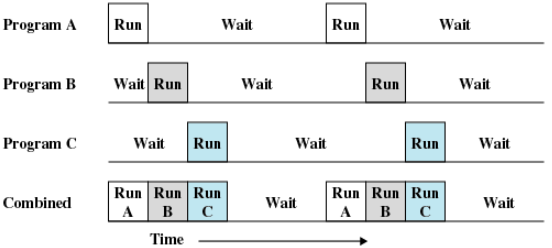
\includegraphics[width=0.5\textwidth]{multiprogramming.png}
\end{center}

Time-sharing is the natural extension of multiprogramming. It allows multiple users to interact with a computer system simultaneously.  Whereas a multiprogramming batch system aims to maximize CPU usage, a time-sharing system aims to minimize the response time of a system to the inputs of multiple users.  A time-sharing system must use multiprogramming and CPU scheduling to achieve this.  Despite this difference in goals between time-sharing and multiprogramming systems, time-sharing systems tend to also achieve high CPU usage since time-sharing is a functionality built on top of multiprogramming and CPU usage is not entirely tangential to minimizing response time.

\newpage

\section*{Question 2}

As stated in my answer to Question 1, a uniprogramming system is a system that can only run and manage a single process at once.  So, once a process starts, even if it doesn't use the CPU, the CPU will not execute the instructions of any other process until that process finishes.  This means that jobs A, B, and C will run one after the other.  Therefore, the time taken to finish the three jobs on a uniprogramming system is given by

$$3 \cdot (2\text{ms} + 10\text{ms} + 4\text{ms}) = 48\text{ms}$$

As stated in my answer to Question 1, a multiprogramming system is one that can manage multiple processes at once - whether or not it can actually execute multiple instructions in parallel.  This means that while one process is waiting on IO, the CPU will execute the instructions of another process. We assume that all IO can be done in parallel.  Therefore, the time taken by a multiprogramming system to complete the three jobs, A, B, and C is given by

$$(2 + 2 + 2)\text{ms} + (10 - 4)\text{ms} + (4 + 4 + 4)\text{ms} = 24\text{ms}$$

$(2 + 2 + 2)$ is the time needed for all three jobs to do their first round of computing. $(10 - 4)$ is the time needed to wait for job A to finish its 10s IO which it started 4 seconds before job C finished its first round of computing. $(4 + 4 +4)$ is the time needed for all three jobs to finish their second round of computing. \\

It should be noted that my calculations assume that computing cannot happen in parallel.  If the CPU could execute instructions in parallel, the time needed for all three jobs would just be $2 + 10 + 4 = 16$, since all three jobs could run start-to-finish at the same time.

\section*{Question 3}

\begin{minted}[linenos]{c}
#include <stdio.h>
#include <unistd.h>
#include <fcntl.h>

int main()
{
    close(1); // close stdout
    open("redirect.txt", O_WRONLY, O_CREAT); // open redirect.txt
    printf("A simple program output.");
    return 0;
}
\end{minted}

Calling \mintinline{c}{close(1)} closes the connection to {stdout} and removes file descriptor 1 from the process's list of file descriptors.  Then, calling \mintinline{c}{open("redirect.txt", O_WRONLY, O_CREAT)} opens a connection to the file \mintinline{c}{redirect.txt} and puts the file descriptor to it in the slot where we just removed the file descriptor for \mintinline{c}{stdout}.  The flags \mintinline{c}{O_WRONLY} and \mintinline{c}{O_CREAT} mean that the connection to \mintinline{c}{redirect.txt} is 'write-only' and that \mintinline{c}{redirect.txt} will be created if it doesn't already exist.

\end{document}
